\section{Experimental Methodology}%
\label{sec:methodology}

We evaluate the effectiveness of our approach in three case
studies. In the first, we apply our methodology to a suite of
established compiler analysis tasks. These serve as demonstrations of
the representational power of our approach and highlight the
limitations both in prior machine learning approaches and in current
MPNNs. The second case study then applies the approach to the
challenging real-world optimization task of heterogeneous device
mapping, comparing the performance of our model against
state-of-the-art machine learning-based approaches. Finally, we apply
our approach to the task of classifying algorithms from unlabelled
implementations. This section describes the methodology used to
construct these experiments: the datasets used, the model parameters,
and training regimes.


\subsection{Case Study A: Compiler Analyses}

We construct a benchmark suite of traditional compiler analysis tasks
to evaluate the representational power of our approach.  We chose a
diverse set of tasks to capture a mixture of both forward and backward
analyses, and control-, data-, and procedure-sensitive analyses. Our
goal is not to suggest that machine learning should replace the
existing implementations of these standard algorithms which can be
found in any compiler, but rather, if a machine learning system is
\emph{not} capable of producing these analyses, it stands to reason
that performance on downstream tasks which depend on these analyses
will suffer.

\subsubsection{Benchmark Analyses}

We selected five traditional compiler analyses to use as benchmarks
for evaluating the representational power of our approach.

\paragraph{(I) Reachability} Control reachability is a fundamental
compiler analysis which determines the set of statements that can be
reached from a particular starting statement. Given $\text{succ}(n)$,
which returns the control successors of statement $n$, the set of
reachable statements starting at root $n$ can be found using forward
analysis:

\begin{equation}
  \text{Reachable}(n) = \{n\} \cup \left( \bigcup_{s \in \text{succ}(n)} \text{Reachable}(s) \right)
\end{equation}

\paragraph{(II) Dominator trees} Statement $n$ dominates statement $m$
if every control flow path to $m$ passes through $n$. A dominator tree
is the set of all nodes that dominate the statment at a particular
program point. Like reachability, this analysis only requires
propagation of control flow, but unlike reachability, dominator trees
are typically constructed using backward
analysis~\cite{Lengauer1979,Blazy2015}:

\begin{equation}
  \text{Dominators}(n) = \{n\} \cup \left( \bigcap_{p \in \text{pred}(n)} \text{Dominators}(p) \right)
\end{equation}

Where $\text{pred}(n)$ which returns the control predecessors of
statement $n$.

\paragraph{(III) Live-out variables} A variable $a$ is live-out of
statement $n$ if there exists some control successor of $n$ that uses
$a$. Given $\text{uses}(n)$, which returns the operand variables of
$n$, and $\text{defs}(n)$, which returns defined variables, the
live-out variables can be computed forwards using:

\begin{equation}
  \text{LiveOut}(n) = \bigcup_{s \in \text{succ}(n)} \text{uses}(s) \cup \big(  \text{LiveOut}(s) - \text{defs}(s) \big)
\end{equation}

\paragraph{(IV) Data dependencies} The data dependencies of statement
$n$ is the set of predecessor statements that must be evaluated to
produce the operands of $n$. Computing data dependencies requires data
sensitivity and is computed backwards:

\begin{equation}
  \text{DataDep}(n) = \text{defs}(n) \cup \left( \bigcup_{p \in \text{defs}(n)} \text{DataDep}(p) \right)
\end{equation}

Where $\text{defs}(n)$ returns the statements that produce operands of
$n$.

\paragraph{(V) Global Common Subexpressions} The identification of
common subexpressions is an important analysis for optimization. For
compiler IRs we define a subexpression as a statement and its
operands, ordered by either their position (for non-commutative
operations), or lexicographically (for commutative operations). We
thus formulate the common subexpression problem as, given a statement
(which forms part of a subexpression), label any other statements in
the program which compute the same subexpression. This is an
inter-procedural analysis, though operands must obey their
scope. Common subexpressions are typically identified using available
expression analysis:

\begin{equation*}
\text{Avail}(n) = \text{uses}(n) \cup \left( \bigcap_{p \in \text{pred}(n)} \text{Avail}(p) \right) - \text{defs(n)}
\end{equation*}

Where $\text{uses}(n)$ return the expressions used by statement $n$,
and $\text{defs}(n)$ returns the expressions defined by $n$.


\subsubsection{Datasets}

We assembled a large corpus of real-world LLVM-IRs from a variety of
sources, summarized in Table~\ref{table:corpus}. We selected popular
open source software projects that cover a diverse range of domains
and disciplines, augmented by uncategorized code mined from popular
GitHub projects using the methodology described by Cummins et
al.~\cite{Cummins2017a}. Our corpus comprises a range of source
languages (C, C++, Fortran, Haskell, OpenCL, and Swift) and exceeds
250k files. We de-duplicated the corpus first at the source level,
then again after lowering to LLVM-IR. Lowering from source to IR was
performed using the inst2vec methodology~\cite{Ben-nun2018}, in which
an optimization level is chosen randomly per-file.

\begin{table}
  \centering%
  %+------------------------------------------------------------+----------+------------+-------------+------------+-----------------+-----------------+---------------+
%| source_name                                                | language | file_count | graph_count | line_count | statement_count | statement_count | branch_factor |
%+------------------------------------------------------------+----------+------------+-------------+------------+-----------------+-----------------+---------------+
%| blas-3.8.0                                                 | fortran  |        300 |          83 |     114083 |          165718 |          326782 |    1.92486627 |
%| github.com/av-maramzin/SNU_NPB:NPB3.3-SER-C                | c        |        122 |           3 |       1239 |             975 |            1815 |    1.64823333 |
%| linux-4.19                                                 | c        |      13920 |        3848 |   11164045 |         6935620 |        14005386 |    1.91736788 |
%| opencv-3.4.0                                               | cpp      |        442 |         110 |     283008 |          377520 |          751432 |    1.91927636 |
%| pact17_opencl_devmap                                       | opencl   |        256 |          76 |      59241 |          105652 |          204598 |    1.75749474 |
%| sqlite:////var/phd/datasets/github/repos_by_lang/c.db      | c        |      43618 |       11732 |   10370757 |        10791095 |        20878352 |    1.73002717 |
%| sqlite:////var/phd/datasets/github/repos_by_lang/opencl.db | opencl   |       5302 |        1345 |    1848119 |         3033871 |         6794770 |    1.72519063 |
%| sqlite:////var/phd/datasets/github/repos_by_lang/swift.db  | swift    |       4719 |         514 |      63970 |           75830 |          202087 |    1.04556031 |
%| tensorflow                                                 | cpp      |       1986 |         396 |    2326580 |         2454937 |         4884154 |    1.92428460 |
%+------------------------------------------------------------+----------+------------+-------------+------------+-----------------+-----------------+---------------+
\renewcommand{\arraystretch}{1.55}
\footnotesize
\begin{tabular}{L{3.35cm} L{1.45cm} L{2.75cm} | r r R{1.69cm} R{1.6cm}}
  & \textbf{Source language} & \textbf{Domain} & \textbf{IR files} & \textbf{IR lines} & \textbf{Avg. vertices / IR} & \textbf{Avg. edges / IR}\\
  \hline
  BLAS 3.8.0 & Fortran & Scientific Computing & 300 & 345,613 & 1,664 & 3,276\\
  \hline
  Linux 4.19 & C & Operating Systems & 13,851 & 41,332,089 & 1,857 & 3,760 \\
  \hline
  OpenCL Benchmarks~\cite{Cummins2017b} & OpenCL & Benchmarks & 256 & 149,779 & 1,027 & 1,970 \\
  \hline
  OpenCV 3.4.0 & C++ & Computer Vision & 400 & 1,168,758 & 3,761 & 7,442\\
  \hline
  POJ-104~\cite{Mou2016} & C++ & Standard Algorithms & 182,815 & 64,518,837 & 312 & 569 \\
  \hline
  Tensorflow~\cite{Abadi} & C++ & Machine learning & 1,584 & 8,444,443 & 5,786 & 11,482 \\
  \hline
  \multirow{4}{*}{GitHub} & C & \multirow{4}{*}{Various} & 42,880 & 89,356,570 & 927 & 1,794\\
                  & Haskell & & 1,371 & 6,745,312 & 4,705 & 7,518\\
                  & OpenCL & & 5,188 & 10,472,388 & 2,299 & 5,132 \\
                  & Swift & & 1,783 & 205,140 & 134 & 371 \\
  \hline
  \textbf{Total} & --- & --- & \textbf{250,428} & \textbf{222,738,929} & \textbf{153,426,059} & \textbf{294,685,614} \\
  % \textbf{Total} & --- & --- & $\bm{250,428}$ & $\bm{2.2 \times 10^8}$ & $\bm{1.5\times10^8}$ & $\bm{3.0\times10^8}$ \\
  \hline
  % node count =\textbf{Avg. 2,247} & edge count = \textbf{Avg. 4,331}
\end{tabular}
%
  \vspace{.5em}
  \caption{%
    The ten sources of LLVM-IR used to produce datasets for evaluating
    data flow analyses. Our corpus comprises six programming languages
    from functional to imperative, high-level to accelerators. The
    software covers a broad range of disciplines from compilers and
    operating systems to traditional benchmarks, machine learning
    systems, and unclassified code downloaded from popular open source
    repositories.%
  }%
  \label{table:corpus} %
\end{table}

We generated a single \textsc{ProGraML} representation for each of the
LLVM-IRs, taking an average of 31 ms per IR. Our corpus of unlabeled
graphs totals 153M vertices and 295M edges, with an average of 616
vertices per graph with 472 unique vertex representations, and 1183
edges with a maximum edge position of 355 (a large \texttt{switch}
statement found in a Tensorflow compute kernel).

We produced labeled graphs from the unlabeled corpus by computing
ground truth labels for each of the analysis tasks using a traditional
analysis implementation.  For each of the five tasks, and for every
unlabeled graph in the corpus, we produce $n$ labeled graphs by
selecting unique source vertices $v_{0} \in V$, where $n$ is
proportional to the size of the graph:
\begin{equation}
n = \min \left( \left\lceil \frac{|V|}{10} \right\rceil, 10 \right)
\end{equation}
Each instance in the datasets consists of an input graph in which the
source vertex is indicated using the \emph{vertex selector}, and an
output graph with the ground truth labels used for training or for
evaluating the accuracy of model
predictions. Figure~\ref{fig:dataflow_examples} illustrates an example
input-output instance for each of the five tasks.

We divided the datasets randomly using a 3:1:1 ratio for training,
validation, and test instances. The same random allocation of
instances was used for each of the five tasks. Where multiple labeled
graphs were derived from a single IR, instances derived from the same
IR were allocated to the same split.

\begin{figure}
  \centering
  \begin{subfigure}{.19\linewidth}
    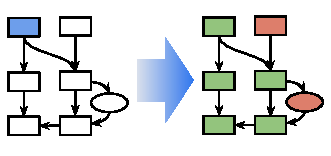
\includegraphics[width=\linewidth]{images/dataflow/A_reachability}%
    \caption{\textsc{Reachability}.}
    \label{subfig:dataflow_reachability}
  \end{subfigure}
  \hfill
  \begin{subfigure}{.19\linewidth}
    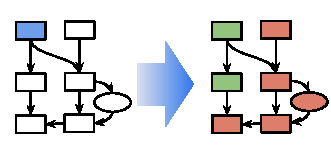
\includegraphics[width=\linewidth]{images/dataflow/B_domtree}%
    \caption{\textsc{Domtree}.}
    \label{subfig:dataflow_domtree}
  \end{subfigure}
  \hfill
  \begin{subfigure}{.19\linewidth}
    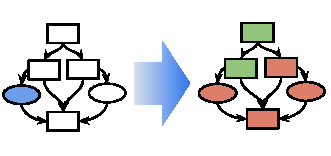
\includegraphics[width=\linewidth]{images/dataflow/C_datadep}%
    \caption{\textsc{DataDep}.}
    \label{subfig:dataflow_datadep}
  \end{subfigure}
  \hfill
  \begin{subfigure}{.19\linewidth}
    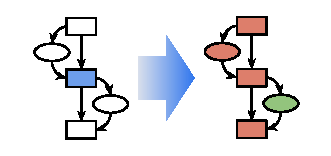
\includegraphics[width=\linewidth]{images/dataflow/D_liveness}%
    \caption{\textsc{Liveness}.}
    \label{subfig:dataflow_liveness}
  \end{subfigure}
  \hfill
  \begin{subfigure}{.19\linewidth}
    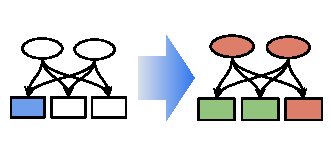
\includegraphics[width=\linewidth]{images/dataflow/E_subexpressions}%
    \caption{\textsc{Subexpressions}.}
    \label{subfig:dataflow_subexpressions}
  \end{subfigure}
  \caption{%
    Example input-output graphs for each of the five benchmark
    compiler analyses. A single vertex is randomly selected from the
    input graph to represent the starting program for computing the
    analysis results, indicated using the \emph{vertex selector}. The
    output graphs contain binary labels for each of the graph vertices
    after the analysis has completed. As a supervised classification
    task, the goal of the model is to predict the output vertex labels
    given the input graph. These small graphs are for illustrative
    purposes, the LLVM-IR graphs in our real-world corpus contain an
    average 616 vertices and 1,183 edges.%
  }%
  \label{fig:dataflow_examples}%
\end{figure}

\subsubsection{Models}%
\label{subsubsec:dataflow_models}

\paragraph{LSTM Baseline} As no prior work offers the expressiveness
required to perform the per-statement and per-variable classification
required for these analysis tasks, we extended
DeepTune~\cite{Cummins2017b}, a state-of-the-art deep learning
framework for whole-program classification, to enable per-statement
classification. In DeepTune, an OpenCL program is first tokenized and
mapped to a sequence of embedding vectors which are then processed
through a sequential LSTM model. The final state of the LSTM is
optionally concatenated with program-level features, then fed through
a fully connected neural network to produce a program-level
classification.

Figure~\ref{figure:lstm_node_level} shows how we extended this
approach for statement-level classification of LLVM-IR. We first
replaced the OpenCL tokenizer using one derived from LLVM IR,
resulting in a 179-element vocabulary. To adapt the approach for
performing statement-level classification, we group embedding vectors
by their source statement before using element-wise summation to merge
embedding vectors.

We use the same models parameters as in the original
work~\cite{Cummins2017b} --- 64-dimensional embedding vectors trained
jointly, with 64 sequences per batch, padded and truncated to the same
length. As LLVM IR is more verbose than OpenCL, the sequences are
significantly longer requiring greater device memory during training
and inference. This is a common issue with recurrent neural networks,
as sufficient memory is required to store both the intermediate
results of the forward pass and the gradients during
training~\cite{Ben-Nun2019a}. We found that a sequence length of 5,000
was the maximum that our experimental platform allowed. Where
sequences exceed this length, they are truncated, and the model
outputs padded with zeros to match the expected shape.


\begin{figure}
    \centering %
    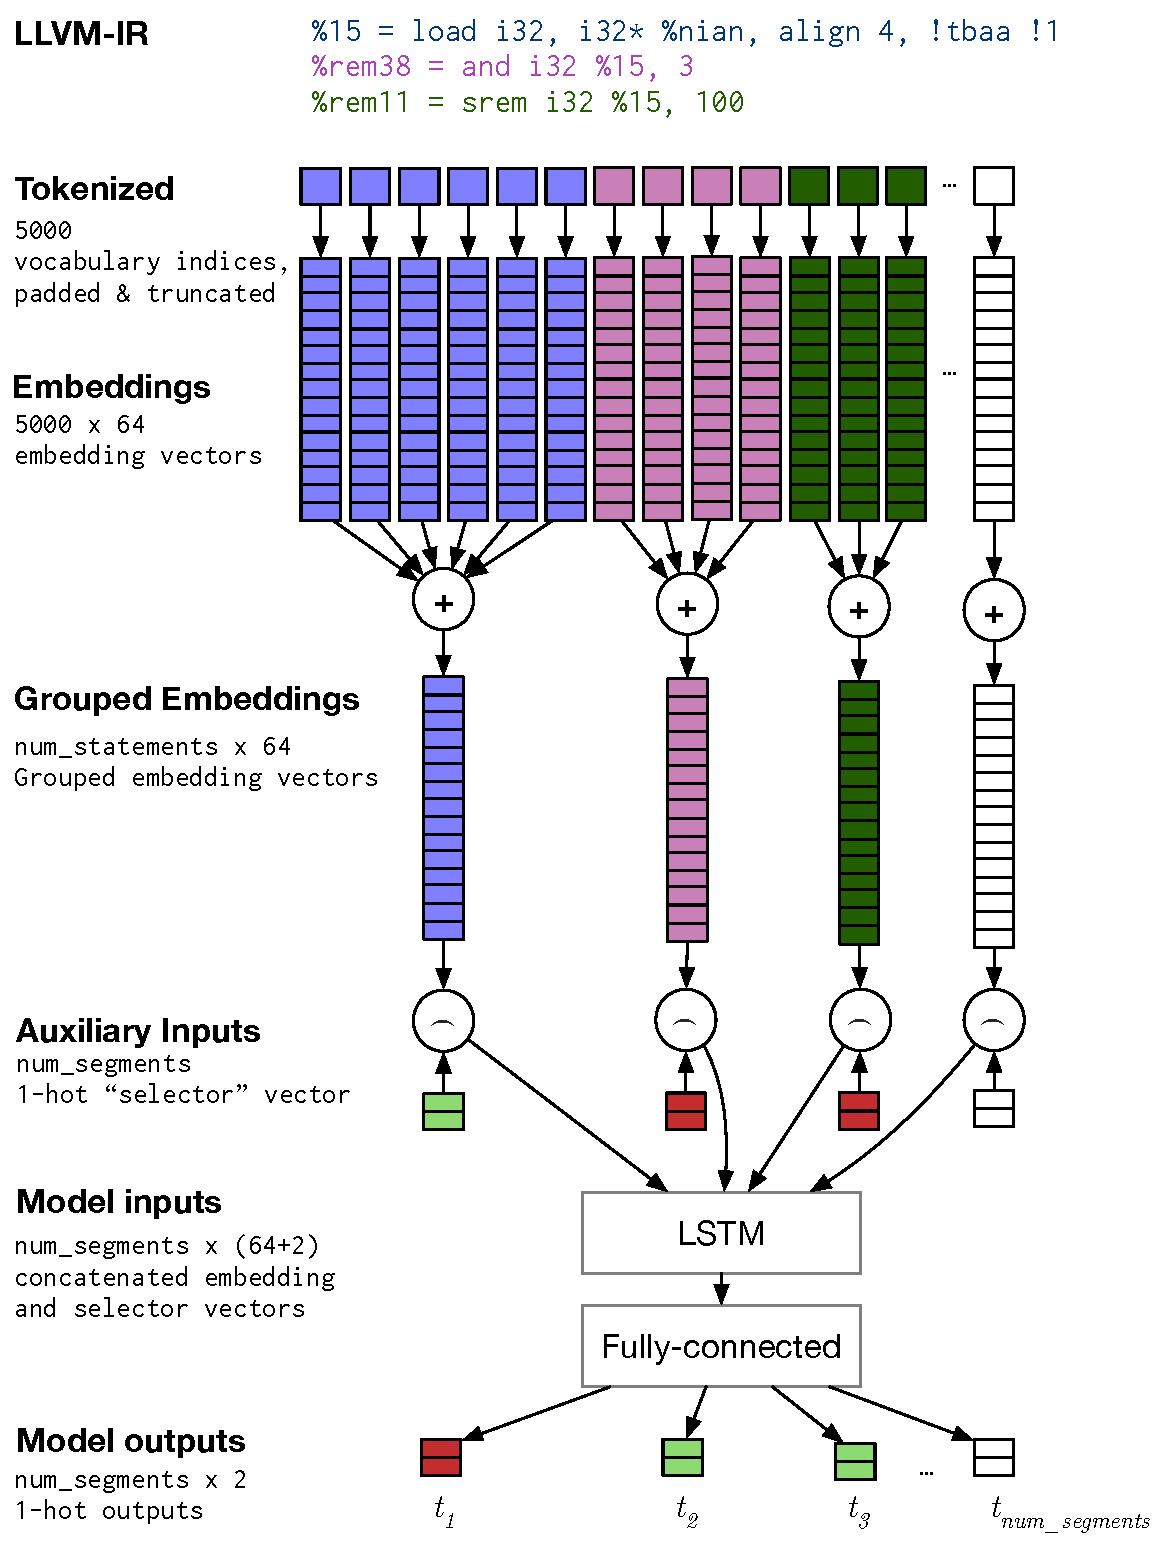
\includegraphics[width=.62\columnwidth]{images/lstm_node_level}%
    \caption{%
      Extending DeepTune~\cite{Cummins2017b} to perform per-statement
      classification of an LLVM-IR. In the original work, the latent
      representation of the entire program token sequence was used for
      program-level classification, we enable classification of
      arbitrary token groupings so that we can perform statement-level
      classification of a program. In the above diagram, $+$ denotes
      element-wise summation, and $\frown$ denotes vector
      concatenation.%
    }%
    \label{figure:lstm_node_level}%
\end{figure}

\paragraph{ProGraML} We use the model design outlined in
Section~\ref{sec:graph-based-machine-learning} for each of the
compiler analysis tasks. While we use the vocabulary of inst2vec, we
do not use the pre-trained embeddings, instead initializing the
embeddings randomly and training jointly.

Message Passing Neural Networks typically use a small number of
propagation steps out of practical consideration for time and space
efficiency~\cite{Gilmer2017,Li2015a}, and address problems on smaller
graphs than used in this work~\cite{Allamanis2017b}. For a large class
of monotone data flow analysis problems, however, it is known that up
to $d(G) + 3$ passes over the graph are required, where $d(G)$ is the
\emph{loop connectedness} of $G$~\cite{Cooper2003,Kam1977}.  The
\emph{loop connectedness} captures the notion of loop-nesting depth in
a program and is therefore a program-dependent, but generally
unbounded quantity\footnote{Given any depth-first spanning tree (DFST)
  of $G$, backward edges are defined as edges in $G$ that connect a
  node to one of its ancestors in the DFST and $d(G)$ is the maximum
  number of backwards edges in any acyclic path in $G$.}.

We address this challenge with \textsc{ProGraML} by iterating for a
fixed number $T$ of message passing steps for training and inference
and excluding from the test set graphs for which a traditional
implementation of the analysis task requires greater than $T$
iterations to solve. For the experiments in this work we set $T = 30$,
leading to 12.56\% of the graphs in the corpus to be excluded across
the five tasks. For fairness, we also excluded these graphs from
evaluation of the LSTM baseline.


\subsubsection{Training Details and Parameters}
All models were trained in an end-to-end fashion with the Adam
optimizer \cite{Kingma2015} using the default configuration and
learning rate $0.001$. We trained the models on a NVIDIA GTX 1080
GPU-equipped machine in increments of 10k graphs, testing on a 20k
validation set at each checkpoint. Training terminated after six
hours, or if accuracy on the validation set reached 99.99\%. After
training completed we selected the checkpoint with the highest
accuracy on the validation set to use for testing.


\subsection{Case Study B: Heterogeneous Device Mapping}

We apply our methodology to the challenging domain of heterogeneous
device mapping (\textsc{DevMap}). Given an OpenCL kernel and a choice
of two devices to run it on (CPU or GPU), the \textsc{DevMap} task is
to predict the device which will provide the best performance. We
chose this problem as it has received significant prior attention,
with previous approaches using both hand-engineered
features~\cite{Grewe2013} and sequential models~\cite{Cummins2017b,
  Ben-nun2018}.

\subsubsection{Datasets}

We used the dataset of~\cite{Cummins2017b}, which provides labeled
CPU/GPU instances for 256 OpenCL kernels sourced from seven benchmark
suites on two combinations of CPU/GPU pairs. The \emph{AMD} set uses
an Intel Core i7-3820 CPU and AMD Tahiti 7970 GPU; the \emph{NVIDIA}
set uses an Intel Core i7-3820 CPU and an NVIDIA GTX 970 GPU. Each
dataset consists of 680 labeled instances derived from the 256 unique
kernels by varying dynamic inputs.

\subsubsection{Models}%
\label{subsubsection:devmap_models}

We compare ProGraML with four approaches: First, with a static
baseline that predicts the mode device of the dataset
distribution. Second, with DeepTune~\cite{Cummins2017b}, which is a
sequential LSTM model at the OpenCL source level. Third, to isolate
the impact of transitioning from OpenCL source to LLVM-IR, we evaluate
against a new DeepTune$_{\text{IR}}$ model, which adapts DeepTune to
using tokenized sequences of LLVM-IR as input instead of OpenCL
tokens, using the vocabulary described in
Section~\ref{subsubsec:dataflow_models}. Finally, we compare against
the state-of-the-art approach NCC~\cite{Ben-nun2018}, which replaces
the OpenCL tokenizer with a sequence of 200-dimensional embeddings,
pre-trained on a large corpus of LLVM-IR using a skip-gram model.


\subsubsection{Training Details and Parameters}

All neural networks are regularized with Dropout \cite{Hinton2012} for
generalization and Batch Normalization \cite{Ioffe2015a} in order to
be uniformly applicable to vastly different scales of auxiliary input
features. We used $10$-fold cross-validation with rotating 80/10/10
splits by training on 80\% of the data and selecting the model with
the highest validation accuracy, setting aside $1/10$th of the
training data to use for validation. We trained each model for 100
epochs and selected the epoch with the greatest validation accuracy
for testing.


\subsection{Case Study C: Algorithm Classification}

In a third case study, we apply our approach to task of classifying
algorithms. We use the POJ-104~\cite{Mou2016} dataset.  It contains
implementations of 104 different algorithms that were submitted to a
judge system. All programs were written by students in higher
education. The dataset has around 500 samples per algorithm. We
compile them with different combinations of optimization flags to
generate a dataset of overall 240k samples. Approximately 10,000 files
are held out each as a development and test set.


\subsubsection{Models}

We compare with recently published tree-based convolutional neural
networks (TBCNN)~\cite{Mou2016} and NCC~\cite{Ben-nun2018}, which uses
the same approach approach as described in
Section~\ref{subsubsection:devmap_models} on this dataset. To further
test the expressive power of the graph-based representation against
the tree-based (TBCNN) and sequential (NCC) prior work, we present
additional experiments: Graph-based baselines based on
XFG~\cite{Ben-nun2018} and a \textsc{ProGraML} \emph{structure-only}
baseline.

To better understand the qualitative aspects of replacing a
graph-based representation that captures program semantics like
Contextual Flow Graphs~\cite{Ben-nun2018} (XFG) with the more complete
\textsc{ProGraML} representation, we adapted a GGNN~\cite{Li2015a} to
directly predict algorithm classes from XFG representations of the
programs. In contrast to this, Ben-Nun et al.~\cite{Ben-nun2018} used
XFG only to generate statement contexts for use in skip-gram
pre-training. Here, we lift this graphical representation and make it
accessible to a deep neural network directly, as opposed to the
structureless sequential approach in the original work (NCC).

Additionally, we include a \emph{structure-only baseline} of our
\textsc{ProGraML} approach, where only the type of each node
(instruction, variable, or constant) is encoded, refraining completely
from tokenizing statements. We think that algorithm classification is
a problem that lends itself especially well to judging the power of
the representation \emph{structure}, since most algorithms are
well-defined independent of implementation details such as datatypes.

To test the limits of the expressivity of \textsc{ProGraML}, combine
our representation with a powerful 10-layer
Transformer~\cite{Vaswani2017} encoder model, adapted as a graph
neural network for attributed graphs. We induce graph structure by
masking the attention scores in the self-attention layer with the
adjacency matrix of the \textsc{ProGraML} graphs. A new
space-efficient sparse implementation allows processing of graphs with
on the order of $10^5$ vertices. Different edge types are encoded by
introducing separate \emph{key} and \emph{value} projection matrices
into the self-attention layer~\cite{Vaswani2017,Fisches2020}.


\subsubsection{Training Details and Parameters}

The GGNN models were trained with the AdamW~\cite{Loshchilov2019}
optimizer with learning rate
$2.5\cdot 10^{-4}, \beta_1=0.9, \beta_2=0.999, \varepsilon=10^{-8}$
for 80 epochs. Dropout regularization is employed on the graph states
with a rate of $0.2$. The Transformer model uses the same
hyperparameters as the GGNN. Additionally a batch size of 64, Dropout
regularization of 0.2 on the graph states and weight-sharing between
adjacent pairs of layers is employed. The model dimension is equal to
the embedding size (200) and the hidden size of the feed-forward
layers is 512. The self-attention layers use 5
heads~\cite{Vaswani2017}. Overall, the Transformer model has 5.6
million trainable parameters, around 1.7 million of which are in the
embedding layer.
